\section{Pinhole camera}
\label{sec:pinhole_camera}
Pinhole camera is the simplest camera model, where light passes through a tiny hole (from which the name \textit{pinhole camera}) of a box: an inverted image of the scene is projected on the opposite side of the box itself. This effect, known as \textit{camera obscura effect}, was studied since 500 BC (the first writings are back to the chinese Mozi) and it is the underlying principle of the $19^{th}$ century cameras. An example of the geometry of this camera is shown in Figure \ref{fig::pinhole}: as it can be seen, for each 3D point there is only one ray of light that passes through the pinhole. This is an ideal condition which allows to neglect distortions, such as blurring. Furthermore it is free of lenses, a condition that accords you to neglect distortions such as vignetting or radial and tangential distortions.
\begin{figure}[t!]
  \centering
  \begin{minipage}[c]{.48\textwidth}
  	\centering
    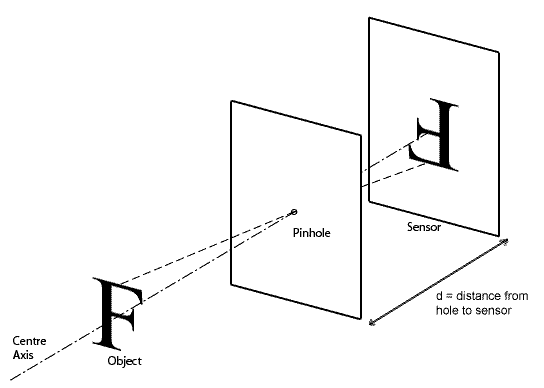
\includegraphics[width=\textwidth]{./images/tech/pinhole.png}
    \caption{The geometry of a \\ pinhole camera}
    \label{fig::pinhole}
  \end{minipage}
  \hfill
  \begin{minipage}[c]{.48\textwidth}
  	\centering
    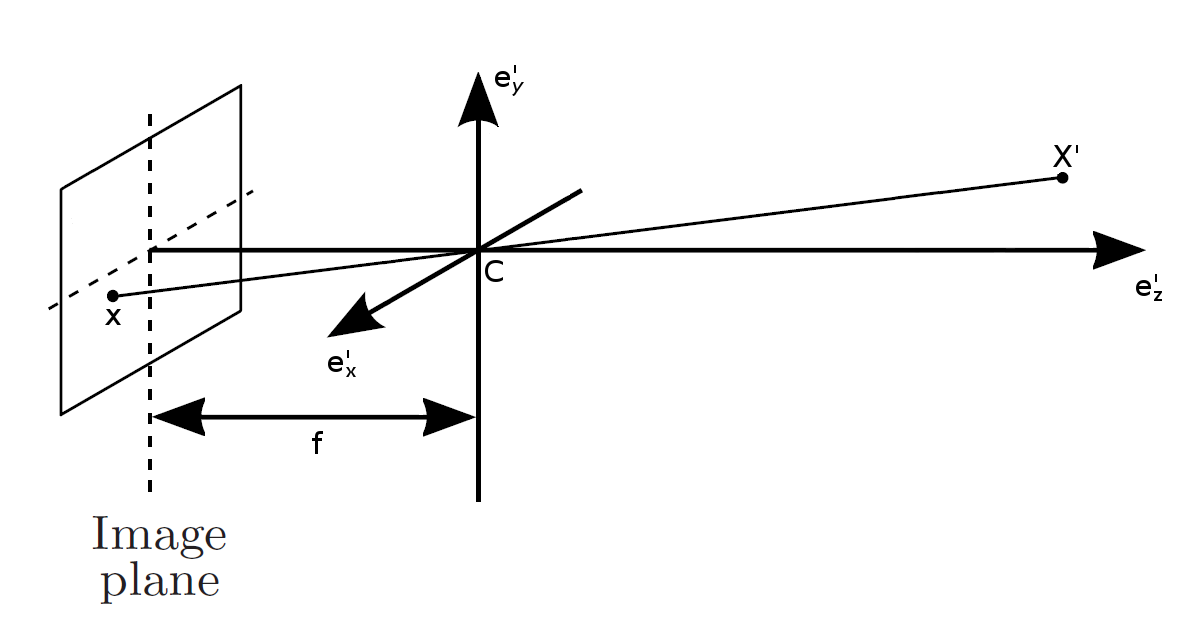
\includegraphics[width=\textwidth]{./images/tech/image_plane.png}
    \caption{Mathematical model}
    \label{fig:math_model}
  \end{minipage}
  %\caption{Examples of different types of occlusions}
  %\label{fig:occlusions}
\end{figure}

Thanks to these simplifications, the mathematical model that describes the relations between the 3D world points and their projections in the image, is very simple. Let's look at the Figure \ref{fig:math_model}. 
% Let us define the \textit{camera coordinate system} $\left(e_x', e_y', e_z' \right)$: the origin $c = \left(0,0,0 \right)$ will represent the so called camera center (i.e. the pinhole).
% We form the line between $X = \left( X_1^w, X_2^w, X_3^w \right)$ and $c$ and intersect it with the plane $z = k$ called \textit{image plane}, to generate a projection $x = (x_1, x_2, k)$ of a scene point $X$. We will refer to $e_Z$ as the \textit{viewing direction}.
% Note that if $k > 0$, the image plane is placed in front of the camera center and the image will not appear upside down. In this case we talk about \textit{virtual image}, but in real models we put $k < 0$. \\
% Since $Xc$ is a direction vector of the viewing ray we can parametrize it by the expression
%  \begin{equation*}
%    c + s(X - c) = sX \qquad s \in \mathds{R}
%  \end{equation*}
% where $sX_3^w = k$ (intersection with the plane $z = k$). Note that this model does not take into account the scene projection from the image plane to the sensor plane. \\
Let $\left(e_x', e_y', e_z' \right)$ be the \textit{camera coordinate system}, centered in $C = \left(0,0,0 \right)$, and let $C$ be the camera center (i.e. the pinhole). Then, let us define the \textit{image plane} as the 2D plane in the world in which the sensor lies. The point 2D $x = (x_1, x_2)$ in the image plane, is related to the 3D world point $X' = (X'_1, X'_2, X'_3)$ through a linear pathway for point $C$. We can parametrize this transformation with the expression:
  \begin{equation}
    \begin{pmatrix} x_1 \\ x_2 \end{pmatrix} = - \frac{f}{X'_3} \begin{pmatrix} X'_1 \\ X'_2 \end{pmatrix}
    \label{eq:image-plane}
  \end{equation}
where $f$ is the \textit{focal length} (the distance from the pinhole to which the rays are focused) of the ideal camera. This is a very simple model, but a point in the image plane does not correspond to a unique point in the world as there are three unknowns on the right hand side. Thanks to the collinearity condition from the points $X'$, $x$ and $C$, the \acs{DLT} (Direct Linear Transformation, an algorithm used to determine a set of variables from a set of similarity relations) is used: it is simple to solve this intersection and to determine this last projection. \\

However, this case is unrealistically simple, because the object and image plane are parallel. In real applications, the point $X$ can lie on a plane that have an arbitrary position and rotation, with respect to the image plane. Let us put this new plane into a \textit{global coordinate reference system} $\left( e_x, e_y, e_z \right)$; all points in the 3D world and all the camera movements will be related to this system.
% In Figure \ref{fig:math_model} we can see how point $X$ is projected in the image plane, but a questions arise: how we can locate $X$ in the world and where image plane is located respecting to the world? To answer to these questions we have to introduce a new \textit{global coordinate reference system} $\left( e_x, e_y, e_z \right)$; all points in the 3D world and all the camera movements will be related to this system.
In this way the projection of the point $X$ in the camera reference system $\left( e_x', e_y', e_z' \right)$ is a simple rotation and translation, that in \textit{homogeneous coordinates} is:
  \begin{equation}
    \label{eq:extrinsic}
    \begin{pmatrix}
      X'_1 \\ X'_2 \\ X'_3
    \end{pmatrix}
    =
    \begin{bmatrix}
      R & t
    \end{bmatrix}
    \begin{pmatrix}
      X_1 \\ X_2 \\ X_3 \\ 1
    \end{pmatrix}
    =
    H
    \begin{pmatrix}
      X_1 \\ X_2 \\ X_3 \\ 1
    \end{pmatrix}
  \end{equation}
where $R$ is a $3 \times 3$ rotation matrix and $t$ a $3 \times 1$ translation vector, and they are referred to as \textit{extrinsic parameters}, while the matrix $H$ is called \textit{homography matrix}. This is the first projection shown in Figure \ref{fig:perspective_projection}.
\begin{figure}[t!]
  \centering
  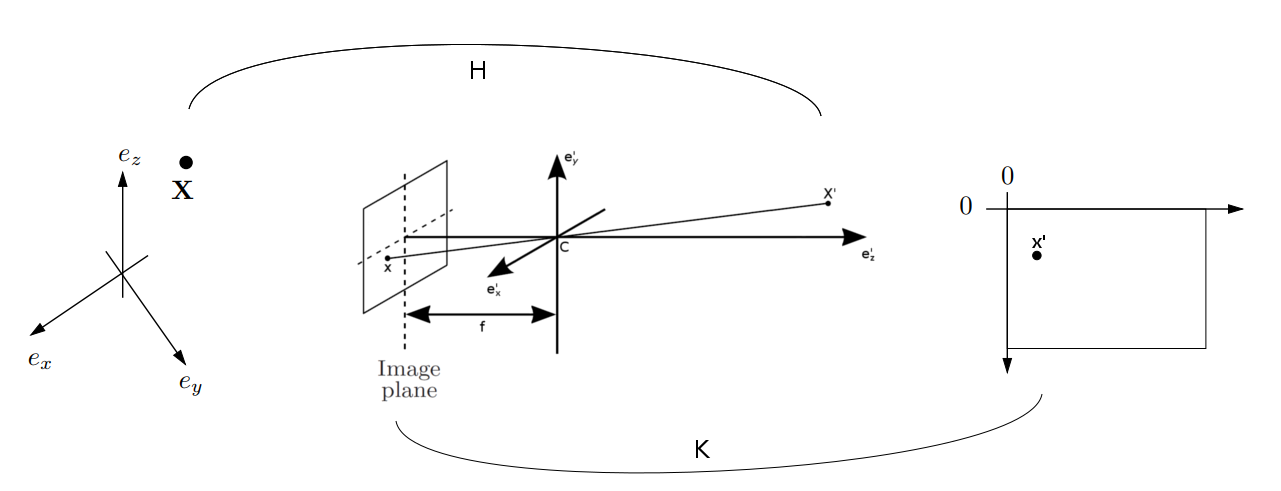
\includegraphics[width=\textwidth]{./images/tech/perspective_projection.PNG}
  \caption{Projection chain from the point $X$ in the world reference system, to $x'$ in the sensor reference system.}
  \label{fig:perspective_projection}
\end{figure} \\

The Equation \ref{eq:image-plane} shown us that the image plane is embedded in $\mathds{R}^3$, so we need to project the point $x'$ in the $\mathds{N}^2$ sensor coordinate system (in pixel unit). This is possible using a $3 \times 3$ matrix $K$ of the \textit{intrinsic parameters}
  \begin{equation*}
    \label{eq:intrinsic_matrix}
    K =
    \begin{pmatrix}
      \gamma_1	& s			& c_x \\
      0			& \gamma_2	& c_y \\
      0			& 0				& 1
    \end{pmatrix}
  \end{equation*}
where $\left( c_x, c_y \right)$ are the coordinates of the point $C$ in the sensor reference system. The pair $\left( \gamma_1, \gamma_2 \right)$ are scale factors that translate the image plane unit ($mm$) into sensor unit ($pixel$). Finally, $s$ is called skew factors, and it forces sensor rows and columns to be perpendicular. These are properties of the used camera and are related to non-ideality of camera construction. The projection (the second in Figure \ref{fig:perspective_projection}) is performed as follow:
  \begin{equation}
    \label{eq:intrinsic}
    \begin{pmatrix}
      x'_1 \\ x'_2 \\ 1
    \end{pmatrix}
    = K 
    \begin{pmatrix}
      x_1 \\ x_2 \\ 1
    \end{pmatrix}
  \end{equation} \\

The chain of all these projections, shown in Figure \ref{fig:perspective_projection}, is called \textit{perspective projection}. A common way to indicate Equations \ref{eq:extrinsic} and \ref{eq:intrinsic} in a single formula through the \textit{homogeneous coordinates} is
  \begin{equation}
    \label{eq:perspective_projection}
    \lambda
    \begin{pmatrix}
      x_1 \\ x_2 \\ 1
    \end{pmatrix}
    = KH
    \begin{pmatrix}
      X_1 \\ X_2 \\ X_3 \\ 1
    \end{pmatrix}
  \end{equation}
where the parameter $\lambda$ takes into account the projection in Equation \ref{eq:image-plane}.

%--------------------------------------------------%
\subsection{Lenses}
\label{subsec:lenses}
As mentioned above, Equation \ref{eq:perspective_projection} does not consider many non-ideality that affect the quality of images acquisitions. 

In Section \ref{sec:pinhole_camera} we introduced the fact that, ideally, only one ray per point passes through the pinhole. If on the one hand this guarantees focus, on the other the impression of the scene in the sensor requires too much time. The increasing of the size of the pinhole allows the passage of light, reducing sensor exposure time. However, in this case the projection of the point on the sensor is the result of the mixing of many light rays, condition that reduces the image sharpness until becomes a continuous smear. Lenses are used to solve this problem.

The role of the lenses is the same as the pinhole: in fact, it allows the passage of light. Their advantage compared to the pinhole is the ability to converge many light rays on a specific point, allowing much more light, and reducing film exposure times. Lens models can be quite complex, so a common practice is considered: the \textit{thin lens approximation}. A thin lens is a lens with a negligible thickness compared to the radii of curvature of its surface. In this way Equation \ref{eq:perspective_projection} remains the same. Despite this, the use of lenses introduces some other issues. \\

The amount of light that impresses the sensors is proportional to the lens diameter. The bigger the diameter is, the more light enters in the camera, but we have to consider also the \textit{magnification}. Magnification is the process of enlarging (factor greater than one) or decreasing (factor less than one, this situation is also called ``minification'') appearance of something. In this case magnification refers to the ability to see more details of the world in a single image. That said, the brightness of the image depends inversely on magnification. A simple way to indicate \textit{aperture} of a lens (the opening through which light travels), is using the \textit{f-number} $K$, defined as
  \begin{equation}
    K = \frac{f}{d}
    \label{eq:fnumber}
  \end{equation}
where $f$ is the lens focal length and $d$ the aperture diameter. As we can see in Equation \ref{eq:fnumber}, $K$ decreasing at increasing of $d$. Thanks to $K$, it is possible to compare lenses, considering image luminosity, focal length and magnification. Note that this is a simple rule with no effects on the Equation \ref{eq:perspective_projection}. \\
  
Another problem is the focus of the lens. While a pinhole camera is permanently on-focus (ideal condition), this is not always valid for a lens. In reality a lens is on focus only at a specific distance: this means that only the point at that distance will be perfectly sharp. All the other points that are out-of-focus are projected on film as circles, called \textit{circles of confusion}. The blur spot shape is due by the aperture shape (that typical is a circle from which the name) and its size increases with the distance from the focus plane. Differently from chemical film, digital sensor are made as a matrix of photosensitive elements (pixels) that convert light in electrical signals; this means that sensors resolution is not infinite. If the circle of confusion is smaller than pixels sizes, we can consider that point on focus. The space range, around the focus plane in which the scene looks reasonably sharp, is called \textit{depth of field} (\acs{DOF}). An example of these effects, common in literature, is shown in Figure \ref{fig:dof}.
%  \begin{wrapfigure}{L}{0.5\textwidth}
%    \centering
%    \includegraphics[width=0.5\textwidth]{./images/dof_txt.jpg}
%    \caption{Example of a very shallow \acs{DOF}.}
%    \label{fig:dof}
%  \end{wrapfigure} \\
  \begin{figure}[t!]
    \centering
    \begin{minipage}[c]{.48\textwidth}
      \centering
 \includegraphics[width=\textwidth]{./images/tech/dof_txt.jpg}
      \caption{Example of a very shallow \acs{DOF}.}
      \label{fig:dof}
    \end{minipage}
    \hfill
    \begin{minipage}[c]{.48\textwidth}
      \centering
 
\includegraphics[width=0.74\textwidth]{./images/tech/airydisk.jpg}
      \caption{Example of an \textit{airy disk}.\\ ~}
      \label{fig:airy-disk}
    \end{minipage}
  \end{figure} \\

The second big advantage of lenses against the pinhole, is the reduction of the diffraction. Diffraction is an effect generated by the interferences of light waves, when the light finds an obstacle or a hole, similar to the size of its wavelength. As the divergent rays now travel to different distances, some of them move out of phase and begin to interfere with each other, adding in some places and partially or completely canceling out in others. This effect, well known in many fields of interest, from electromagnetic to sound, in photography is known as \textit{airy disk} (by his discoverer, George Airy) and it is shown in Figure \ref{fig:airy-disk}. As for \acs{DOF}, even diffraction is negligible if it is smaller than the size of pixels. Diffraction could be present also in the \acs{DOF} of the camera, and depends only by the $f$-number, not by focal length. Lenses reduce this noise on the image, setting their aperture up appropriately. \\

Regardless of the lens model chosen (i.e. thin or thick lenses), their use introduces distortions due to the nature of the lens itself. In geometric optics, a distortion is a deviation from rectilinear projection, caused by small blemishes in the lenses and their alignment. The main optical aberration are two: \textit{radial distortion} and \textit{tangential distortion}. \\
Almost all of the deformation is radial in nature, this is the reason why distortion are more apparent from the center toward the edges of the image. This particular type of distortion is able to change the direction of straight lines, and it is evident during 3D calibration phases, when straight reference objects are seen from the camera as curve. Furthermore, it is often due to the need to expand the field of vision using a camera with short focal distance. Some example of its effects can be seen in Figure \ref{fig:teo-distorsions}. \\
Vice versa, tangential distortion is typically negligible than radial one, then it is ignored in most mathematical models.
  \begin{figure}[h!]
    \centering
 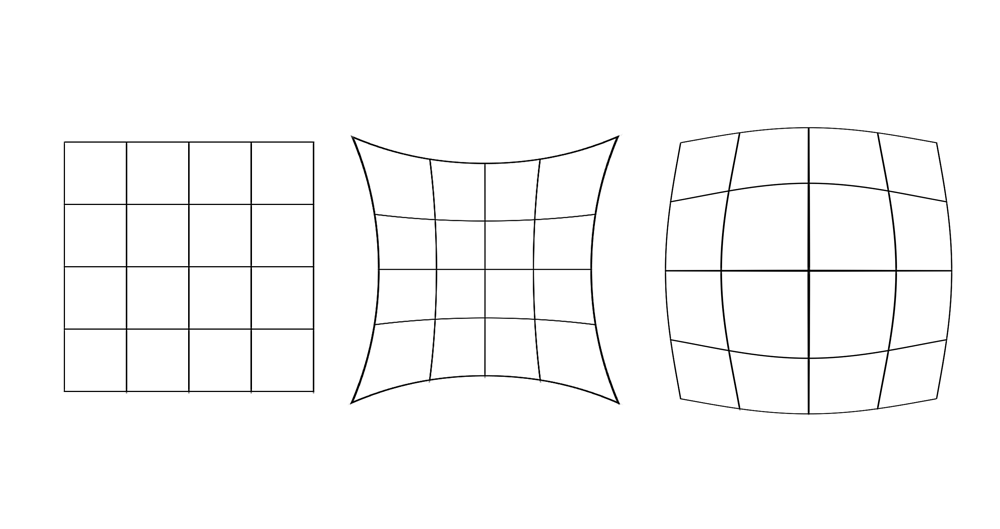
\includegraphics[width=0.9\textwidth]{./images/tech/distorsions.png}
    \caption{Example of radial distortions: on the left distortions free image is shown; in center a \textit{pincushion} aberration; on the right a \textit{barrel} aberration.}
    \label{fig:teo-distorsions}
  \end{figure}

%--------------------------------------------------%
\subsection{Scheimpflug principle}
In the previous subsection we talked about \acs{DOF} and the problem to maintain focus on the whole scene. Furthermore, we dealt with the Figure \ref{fig:dof} to show the result. Anyway, in the figure we can see that the subject lies on a plane not parallel with the sensor plane. Typical cameras and lenses are designed so that sensor plane, lens plane and subject plane are parallel to each other. This makes the focus of the camera very simple but, as said in Subsection \ref{subsec:lenses} talking about the rectilinear projection, the effective focal length depends by the position of the target with respect to the sensor itself. \\

Since the early $20^{th}$ century, the study of rotating the lens with respect to the sensor, and its effects on image acquisition, has been a widespread practice. In $1901$, Carpenter (one of the fathers of cinema) patented the first prototype of the so called ``view camera'' \cite{pat:carpentier}. From these studies, the Captain T. Scheimpflug patented \cite{pat:scheimpflug} in 1904. With his patent, Scheimpflug was the first to formulate the mathematical problem. The \textit{Scheimpflug principle} is a geometric rule that describes the relations between the sensor plane, then lens plane and the plane of focus when the lens plane is not parallel to the image plane. To achieve this situation, some cameras, such as view cameras, allow to tilt either the lens and the film, relative to the other. \\
  \begin{figure}[b!]
    \centering
    \begin{minipage}[c]{0.49\textwidth}
      \centering
      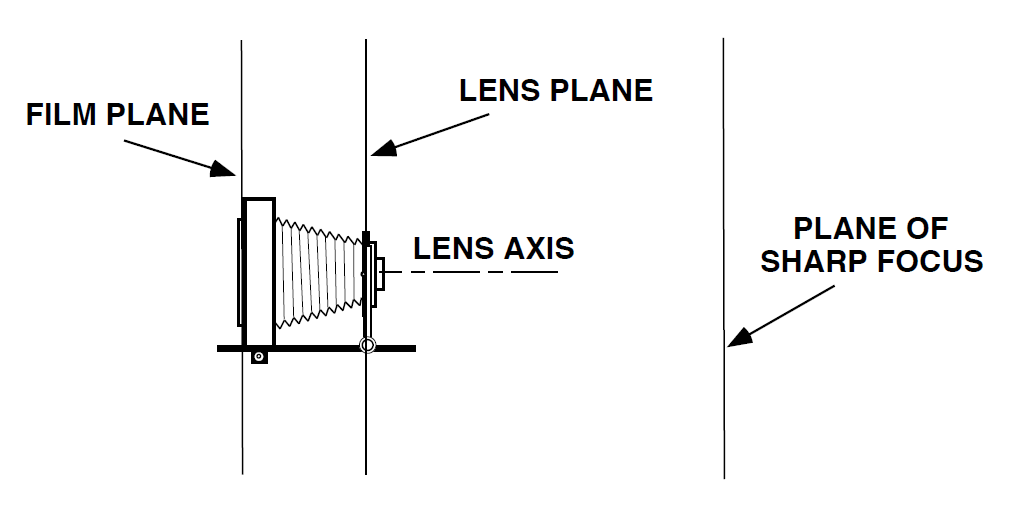
\includegraphics[width=\textwidth]{./images/tech/sch_par.png}
    \end{minipage}
    \hfill\
    \begin{minipage}[c]{0.49\textwidth}
      \centering
      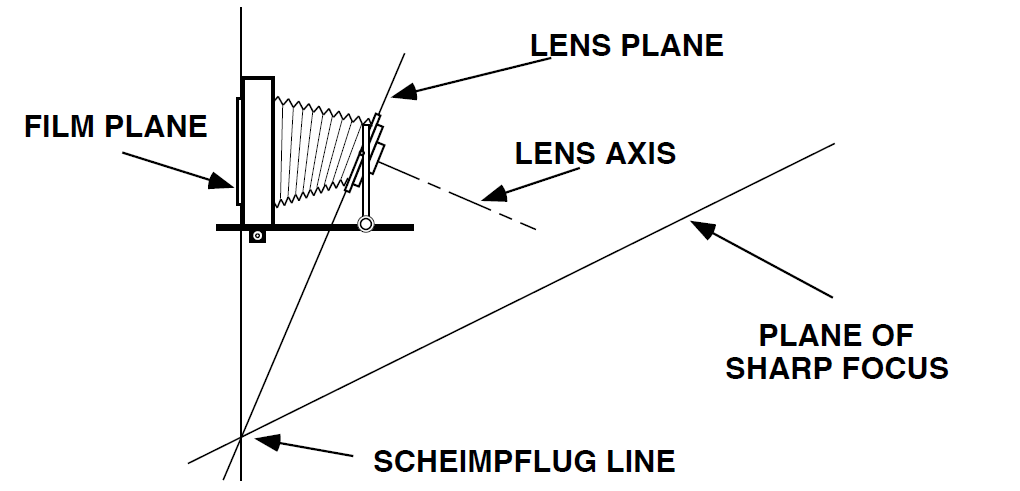
\includegraphics[width=\textwidth]{./images/tech/sch_tilt.png}
    \end{minipage}
    \caption{(On the left) For standard cameras, the sensor, lens and focus planes are parallel to one another. (On the right) For a view camera, tilting lens causes the plane of sharp focus to tilt as well.}
    \label{fig:scheimpflug}
  \end{figure}

This principle asserts that when the lens is tilted, lens plane, image plane and the plane of focus all intersects in a line, called \textit{Scheimpflug line}, as illustrated in Figure \ref{fig:scheimpflug}. In this way, a subject that is not parallel to the sensor can be completely in focus. Nevertheless, this first relation does not give any information about how to tilt the lens to achieve the intended position for the plane of focus. This information arises from the laws of optics, thanks to the \textit{hinge rule}, similar to Scheimpflug one. The required amount of lens tilt is given by the expression:
  \begin{equation*}
    \alpha = \arcsin \left( \frac{f}{J} \right)
  \end{equation*}
where $f$ is the focal length of the lens, and $J$ is the distance from the lens and the \textit{hinge line}. The hinge line is the intersection between a plane parallel with the sensor and passing through the lens one, and the plane of focus. \\
From this principle we can also determine the \acs{DOF} of the camera. It can be demonstrated that the limits of the \acs{DOF} are also planes, that passes through the hinge line, and symmetrical compared to the plane of focus. To be precise, these planes lies at a distance $J$ from the plane of focus, distance measured at the \textit{hyperfocal distance} $H$ from the hinge line \cite{book:ftvc}. The scenario is illustrated in Figure \ref{fig:sch_dof}.
  \begin{figure}[h!]
    \centering
    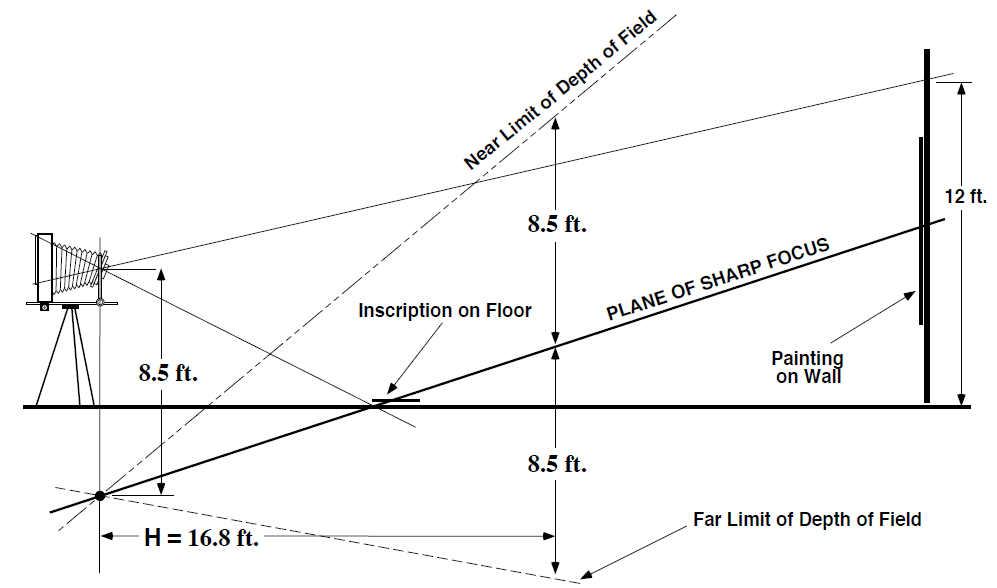
\includegraphics[width=0.8\textwidth]{./images/tech/sch_dof.png}
    \caption{Depth of field in view cameras, with tilted lenses.}
    \label{fig:sch_dof}
  \end{figure}

%--------------------------------------------------%
\subsection{Overview on digital cameras}
\label{subsec:overview-cameras}
To complete the introduction on digital camera we think that it could be useful to linger over some practical aspects, in particular about what concerns manufacturing of the sensor and image acquisitions. \\

In Subsection \ref{subsec:lenses} we introduced the quantization effect due by pixels. If it relaxes the problem of the lens focus, on the other hand it introduces noise in light to image conversion. We briefly analyse the two most popular sensor types on the market: \acs{CMOS} and \acs{CCD} (Charge-Coupled Device).

In \acs{CMOS} sensors, each element has its own signal amplifier: this allows to improve the camera frame rate and to isolate regions of interests via hardware. On the contrary, pixels haven't the same sizes neither the same doping, which reduces the quality of the sensor itself. The latest CMOS sensors on the market are good enough to be used in computer vision, achieving excellent results.

\acs{CCD} are high-scale integration sensors that use only one signal amplifier, ensuring the same amplification constant for each element. However, this requires that sensor rows are converted one by one, by lowering the camera frame rate. Furthermore these sensors give a very small, but non-zero response to a zero input and they saturate for very bright stimuli. In spite of that, they are much less noisy than the CMOS.

These differences are very delicate, specially considering the fields of application of the camera. For example, in laser triangulation systems, the acquired images are dark to highlight the laser light. In situation like this, when the brightness of the image is very low\footnote{In this case we consider source of light with brightness near to the base noise level of the sensor.}, signals amplification offsets are meaningful. The mono-pixel amplifiers in \acs{CMOS} are more noisy and generate less uniform values than \acs{CCD}, resulting in a more homogeneous output. This source of noise is known as \textit{thermal noise}. High quality systems provide different solutions to reduce this effect as much as possible. In Figure \ref{fig:thermal-noise} an example of the noise is shown.
  \begin{figure}[h!]
    \centering
    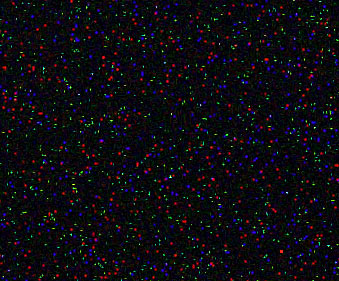
\includegraphics[width=0.5\textwidth]{./images/tech/dark-example.jpg}
    \caption{Example of uncontrolled dark noise in astronomical photography.}
    \label{fig:thermal-noise}
  \end{figure} \\

Another problem due to sensor quantization, is colours acquisition. Each pixel is able to acquire only light signals, resulting in grey scale acquisitions. For this reason sensors needed filters to encode colours. The most widespread is \textit{Bayer's color filter array} (Bayer's \acs{CFA}). A \acs{CFA} is an array in which passband filters are placed, according to a known pattern. In this way each pixel is able to encode only a specific colour. Many algorithms are used to reconstruct the scene; they interpolate signals collected by near pixels and extract the correct colour for each pixel. To perform measures, this is a waste of pixels: the presence of the filter reduces the sensor surface useful to collect world details. For these reasons, grey scale cameras are often used.
